\documentclass[10pt,a4paper]{article}
\usepackage[T1]{fontenc}
\usepackage{lmodern}
\usepackage[margin=18mm]{geometry}
\usepackage[table]{xcolor}
\usepackage{listings}
\usepackage{tabularx}
\usepackage{array}
\usepackage{enumitem}
\usepackage{graphicx}
\usepackage{tcolorbox}
\usepackage{microtype}
\usepackage[hidelinks]{hyperref}
\hypersetup{pdftitle={Phase 2: Port, Review Policies, Test, Inspect},pdfauthor={}}
\graphicspath{{docs/phase2-hw-release/images/}{images/}}
\definecolor{policygray}{gray}{0.93}
\setlength{\parindent}{0pt}
\setlength{\parskip}{5pt}
\setlist{itemsep=2pt,topsep=3pt,leftmargin=1.5em}
\lstset{basicstyle=\ttfamily\footnotesize,columns=fullflexible,
  keepspaces=true,breaklines=true,showstringspaces=false,
  backgroundcolor=\color{policygray},frame=none,
  aboveskip=6pt,belowskip=6pt,xleftmargin=6pt,xrightmargin=6pt}
\newtcolorbox{originalpolicy}{colback=policygray,colframe=policygray,
  boxrule=0pt,arc=0pt,left=7pt,right=7pt,top=5pt,bottom=5pt,
  before skip=6pt,after skip=4pt}
\newcommand{\field}[2]{\item \texttt{#1}: #2}
\begin{document}
\begin{center}
  {\LARGE\bfseries Phase 2: Port, Review Policies, Test, Inspect}
\end{center}
\vspace{-5pt}

We may update these instructions. Please check the
\href{https://github.com/thaddywu/CS239-Phase2/blob/main/phase2-instructions.pdf}{\textbf{latest instructions on GitHub}}
for updates.

In Phase 1, you built an app and described its policies. In Phase 2, you will
review whether our tool preserves your policy intent and test how your app
behaves with runtime enforcement.

\section*{Phase 2A}
Complete Tasks 1--3 on a branch named \texttt{phase2}. Our tool creates a
\emph{ported app}: a version of your app with runtime policy enforcement.
You do not need to inspect the generated implementation.

\subsection*{1. Port}
Create a Git branch named \texttt{phase2} for your submission. Prepare a clean
clone of your original app, with \texttt{app.md} and \texttt{policy.md} committed
in its repository root. Give each policy an ID such as P1 or P2. If a policy
combines several requirements, you may split it into separate lines with IDs
such as P2.1 and P2.2. Make these edits before porting.

Follow Appendix A to install the tool and set the directories and connection file.
Then run:
\begin{lstlisting}
policy-add "$BASE_APP_DIR" "$PORTED_APP_DIR" \
  --connection "$CONNECTION_FILE"
\end{lstlisting}
The tool reads your policy and app code and writes the ported app to
\texttt{PORTED\_APP\_DIR}. It also describes the implemented enforcement in English
and aligns those descriptions with \texttt{policy.md}. These results are saved in
\texttt{PORTED\_APP\_DIR/back-translation/}.

For an overview of the added enforcement, see
\href{https://github.com/thaddywu/CS239-Phase2/blob/main/how-runtime-enforcement-works.pdf}{\textbf{How Runtime Enforcement Works}}.

\subsection*{2. Review Policies}
Compare your original policy with the English descriptions generated from its
implemented enforcement. The review panel shows each original sentence on the
left and the corresponding implemented checks on the right. A sentence may
correspond to several checks.

\begin{lstlisting}
policy-review \
  --back-translation "$PORTED_APP_DIR/back-translation" \
  --policy "$BASE_APP_DIR/policy.md"
\end{lstlisting}

For each sentence, select:
\begin{itemize}
\item \textbf{Fully matches}
\item \textbf{Partly matches}: describe what is missing or different.
\item \textbf{Does not match / not implemented}: describe the difference.
\item \textbf{Not a policy}
\item \textbf{Not sure}: for example, the execution description is unclear.
\end{itemize}
Appendix C shows examples of full and partial matches. These ratings are human
judgments; the tool does not assign your ratings.

\begin{minipage}{\linewidth}
Also classify each policy. You may select multiple categories. The Datalog
rules below are a reference; you do not need to write Datalog.
\par\smallskip

\begingroup
\setlength{\tabcolsep}{6pt}
\begin{tabular}{|p{\dimexpr\linewidth-2\tabcolsep-2\arrayrulewidth\relax}|}
\hline
\textbf{Capability / access control: Who may perform which operations} \\*
\rowcolor{policygray}
\begin{minipage}{\linewidth}
\begin{lstlisting}[xleftmargin=0pt,xrightmargin=0pt]
Can(P, R, E) :- Capability(P, R, E).
Can(P, R, E) :- PrincipalGroup(P, G), Can(G, R, E).
Can(P, Child, E) :- ResourceGroup(Parent, Child), Can(P, Parent, E).
\end{lstlisting}
\end{minipage} \\
\hline
\textbf{Information flow: Where information may go and who may access it} \\*
\rowcolor{policygray}
\begin{minipage}{\linewidth}
\begin{lstlisting}[xleftmargin=0pt,xrightmargin=0pt]
Provenance(D, P) :- Source(P, D).
Provenance(Out, P) :- DependsOn(Out, In), Provenance(In, P).
\end{lstlisting}
\end{minipage} \\
\hline
\textbf{State / lifecycle: Operation ordering, required states and state changes} \\*
\rowcolor{policygray}
\begin{minipage}{\linewidth}
\begin{lstlisting}[xleftmargin=0pt,xrightmargin=0pt]
ReachableState(T, From, To) :- AllowedTransition(T, E, From, To).
ReachableState(T, From, To) :- ReachableState(T, From, Mid),
                             AllowedTransition(T, E, Mid, To).
CanTransition(R, E, From, To) :- ResourceType(R, T),
    ResourceState(R, From), AllowedTransition(T, E, From, To).
\end{lstlisting}
\end{minipage} \\
\hline
\textbf{Other: Enter your own category} \\
\hline
\end{tabular}
\endgroup
\par\smallskip

Click \textbf{Save} to write your judgments to
\texttt{PORTED\_APP\_DIR/review.json}. The panel loads an existing review file so
you can resume. You may also edit the generated \texttt{review.json} directly;
see Appendix B.
\end{minipage}

\subsection*{3. Test Scenarios}
Construct \textbf{5--10 test scenarios} covering normal use, possible policy
violations and boundary cases. Run them on your \textbf{original app}, keeping
its existing protections. You do not need to add new guards.

Record each scenario and its observed run in \texttt{test\_cases.json}:
\begin{itemize}
\field{task}{The concrete task, initial state and user request. For a
conversation, include the user and their permissions, relevant app data and
configuration, prior messages or actions (or that the conversation is new), and
the starting user message.}
\field{expected\_outcome}{The intended final app state and response. Include
concrete values where relevant, such as balances, transfer history and daily-limit usage.}
\field{violated\_policies}{Policies violated in the observed run, with brief
observations and the source of each judgment.}
\field{followed\_policies}{Relevant policies followed in the observed run, with
brief observations and the source of each judgment.}
\field{run\_command}{The command for rerunning the scenario.}
\field{trajectory\_file}{The relative path to the observed run's JSONL trajectory.}
\end{itemize}

\begin{minipage}{\linewidth}
The following example uses a transfer assistant. P1 requires user confirmation
for each transfer; P3 limits daily transfers to \$500.
\begin{lstlisting}
{
  "cases": [
    {
      "task": "Start a new conversation. The user may transfer from S, which has $1,000; recipient R has $0. No transfers today; no fees. The user says: \"Transfer $100 to R.\" Confirm if prompted.",
      "expected_outcome": "After user confirmation, transfer $100 once. Final balances: S $900, R $100; today's transfer total: $100.",
      "violated_policies": [
        ["P1", "The transfer executed without asking for confirmation.", "human-judge"]
      ],
      "followed_policies": [
        ["P3", "The $100 transfer stayed within the $500 daily limit.", "human-judge"]
      ],
      "run_command": "python tests/run_transfer_scenario.py",
      "trajectory_file": "traces/transfer_scenario.jsonl"
    }
  ]
}
\end{lstlisting}
\end{minipage}

\texttt{expected\_outcome} describes the intended result; use the trajectory
to record the actual final state and response. A failed task is still a valid
test. In this example, the balances reach the expected values, but P1 is violated
because the first transfer lacks confirmation.

Each policy-list entry is a triple, \texttt{[policy\_id, observation, judge]}.
Use policy IDs matching \texttt{policy.md} and describe what happened in the run.
Use
\texttt{human-judge}, \texttt{llm-judge}, or \texttt{both} to identify who made
the judgment. Both lists describe the observed run; they may be empty. Omit
policies that were not involved.

Use JSONL for raw trajectories; no fixed event schema is required. Preserve event
order and include user inputs, agent messages, visible LLM outputs, tool-call
arguments and tool results. Include the final app state needed to assess the
outcome. Hidden reasoning is not required.

In your README, explain the original app's environment, how to run each test and
how to read its trajectory. Include scripts, inputs and initial data, and document
manual inputs or actions. A rerun does not need to produce an identical trajectory.

\subsection*{Phase 2A submission}
On your \texttt{phase2} branch, submit:
\begin{itemize}
\item \texttt{ported-app/}: the generated app, including
\texttt{back-translation/} and your completed \texttt{review.json}.
\item \texttt{test\_cases.json}, test scripts, inputs, initial data and original-app trajectories.
\item A README with the original app's commit and the setup and test instructions.
\end{itemize}

\clearpage
\section*{Phase 2B: Test and Inspect}

\textbf{More details coming next Tuesday, November 17.}

\subsection*{4. Run Test Scenarios (required)}
Run your test scenarios on the ported app and save the trajectories. Submit a
report comparing the results with your original app: whether tasks succeed,
whether policy violations are blocked, and whether any violations remain or
legitimate actions are incorrectly blocked.

\subsection*{5. Post-mortem Inspection (optional)}
Import a recorded run into our \textbf{Trajectory Inspector} to view its
trajectory and use predefined questions, such as why a tool call was allowed
or denied. If you try this optional task, include your observations about the
answers in your report.

\clearpage
\section*{Appendix A. Environment and model setup}
The porting runner uses Linux x86\_64, Python 3.10+, Docker and the selected
provider's native coding CLI: Codex for OpenAI or Claude Code for Anthropic.
From the tool repository root, install the packages:
\begin{lstlisting}
python -m pip install -e '.[mcp,test]'
\end{lstlisting}
Build the two execution images following \texttt{docs/porting.md} in the tool
repository.

Set the clean original-app directory, an empty or nonexistent ported-app directory,
and the private model connection file. Keep the app directories separate:
\begin{lstlisting}
export BASE_APP_DIR="/path/to/original-app"
export PORTED_APP_DIR="/path/to/ported-app"
export CONNECTION_FILE="/path/to/private-connection.yaml"
\end{lstlisting}

Copy \texttt{examples/connection.yaml} outside the repository and fill either key:
\begin{lstlisting}
provider: auto
openai:
  apiKey: ""
  modelId: gpt-6.1-sol
anthropic:
  apiKey: ""
  modelId: claude-sonnet-4-6
\end{lstlisting}
With both keys filled, \texttt{auto} selects OpenAI. Set \texttt{provider} to
\texttt{openai} or \texttt{anthropic} to choose explicitly. Model IDs and endpoints
have defaults; overrides belong inside the selected section. JSON connection
files are not accepted. All model-enabled commands use this same YAML file.
Keep credentials out of your submission.

\section*{Appendix B. Editing review.json directly}
Use the file generated by the tool. Keep its version identifiers, sentence IDs
and original text unchanged. Fill in these fields for each sentence:

\begingroup
\small
\renewcommand{\arraystretch}{1.3}
\begin{tabularx}{\linewidth}{@{}>{\raggedright\arraybackslash}p{30mm}>{\raggedright\arraybackslash}X@{}}
\textbf{Field} & \textbf{Values} \\
\hline
\texttt{rating} & \texttt{fully\_correct}, \texttt{partially\_correct},
\texttt{not\_covered}, \texttt{not\_policy}, or \texttt{unsure}; leave empty if unfinished. \\
\texttt{categories} & A list containing \texttt{permission},
\texttt{information\_flow}, \texttt{lifecycle}, \texttt{other}, or \texttt{uncertain}. \\
\texttt{note} & Your observation; required for \texttt{partially\_correct}
and \texttt{not\_covered}. \\
\texttt{other\_category} & Your category name when selecting \texttt{other}.
\end{tabularx}
\endgroup

Use \texttt{uncertain} alone when you cannot classify a policy. Leave categories
empty for \texttt{not\_policy}. If you change \texttt{policy.md} or regenerate
the port, use the corresponding new review file.

\clearpage
\section*{Appendix C. Review examples}
These examples use LabCluster's added policy layer. The English descriptions,
selected ratings and comments shown here were written by humans.

\subsection*{Example 1. Fully matches: resource limits}
\begin{originalpolicy}
\textbf{Policy:} Master may request CPU only, with at most 4 cores, 8 GB and
20 minutes of requested runtime.
\end{originalpolicy}
The submission check reads the requested resources and Master's configured
limits. A non-CPU or over-limit submission is blocked before job creation.
Select \textbf{Fully matches} and \textbf{Capability / access control}.

\begin{center}
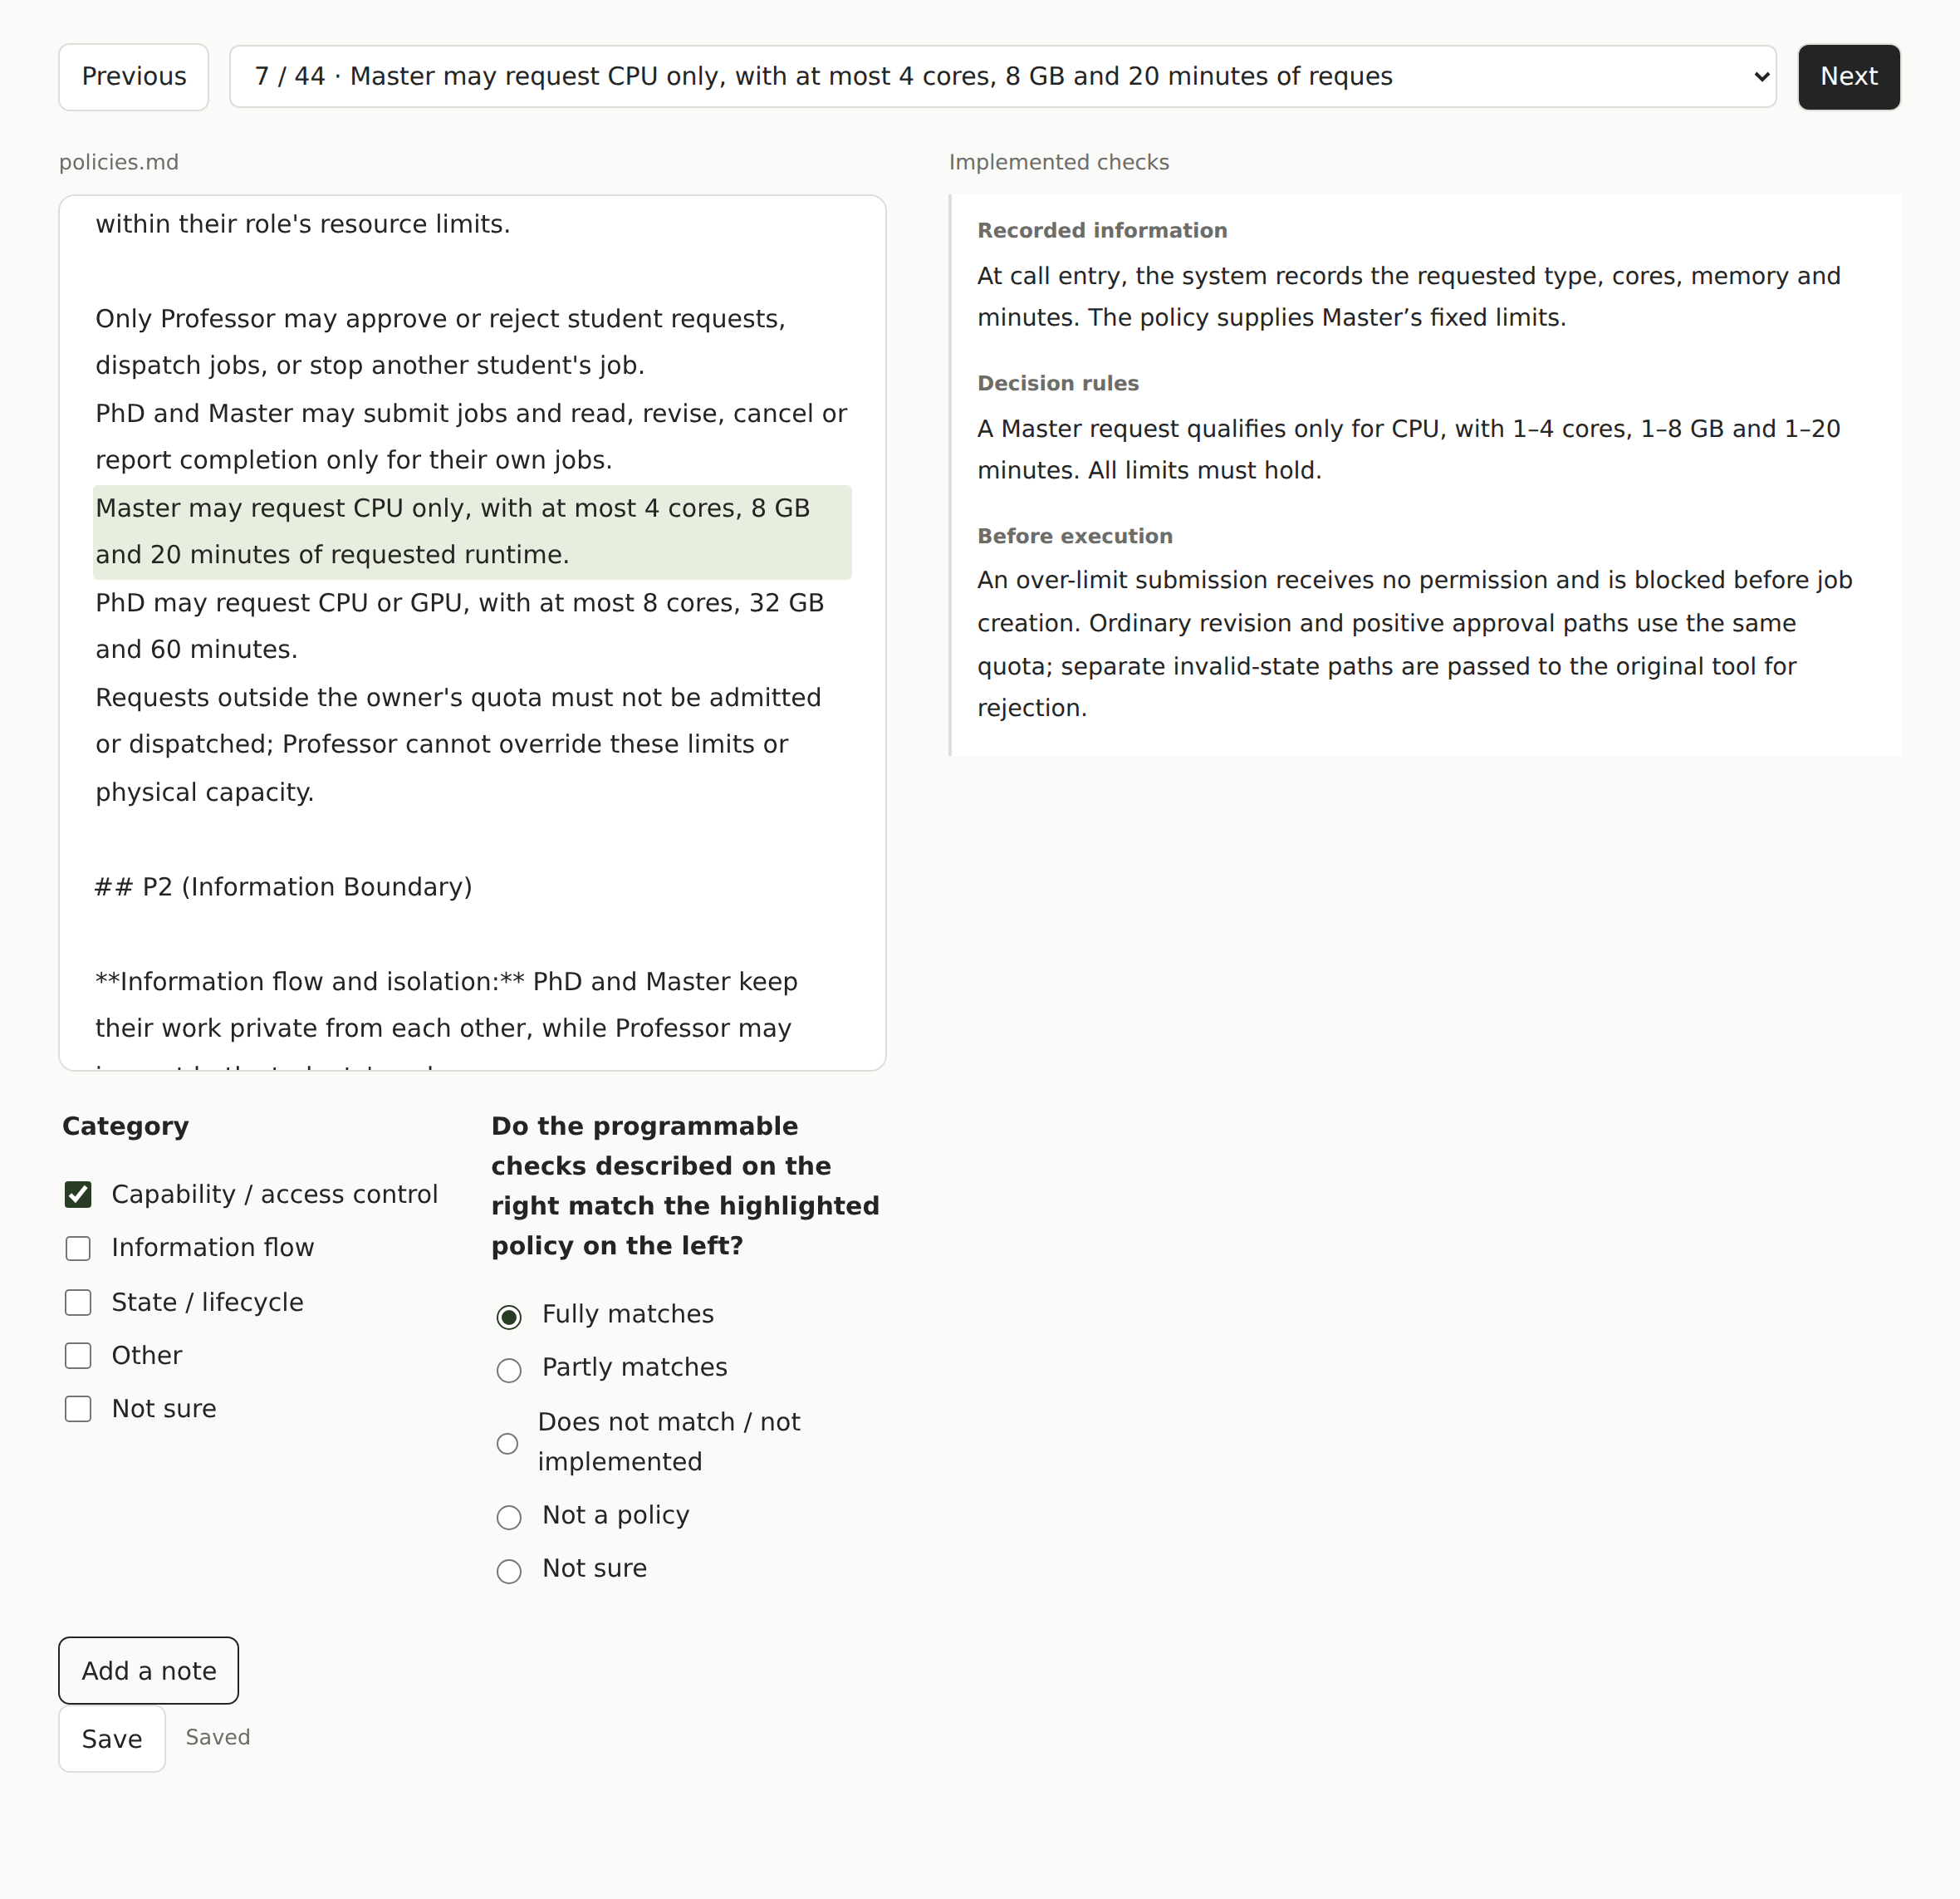
\includegraphics[width=\linewidth,height=0.70\textheight,keepaspectratio]{phase2-review-full.png}
\end{center}

\clearpage
\subsection*{Example 2. Partly matches: private information in messages}
\begin{originalpolicy}
\textbf{Policy:} Neither student may receive the other's private job
specifications, inputs, results, approvals or execution receipts through tools,
model contexts or messages.
\end{originalpolicy}
The message checks compare the referenced job's owner with the sender or
recipient but do not inspect message bodies. A message referencing Master's
own job can still include PhD's private information. Select
\textbf{Partly matches} and \textbf{Information flow}, and describe the gap.

\begin{center}
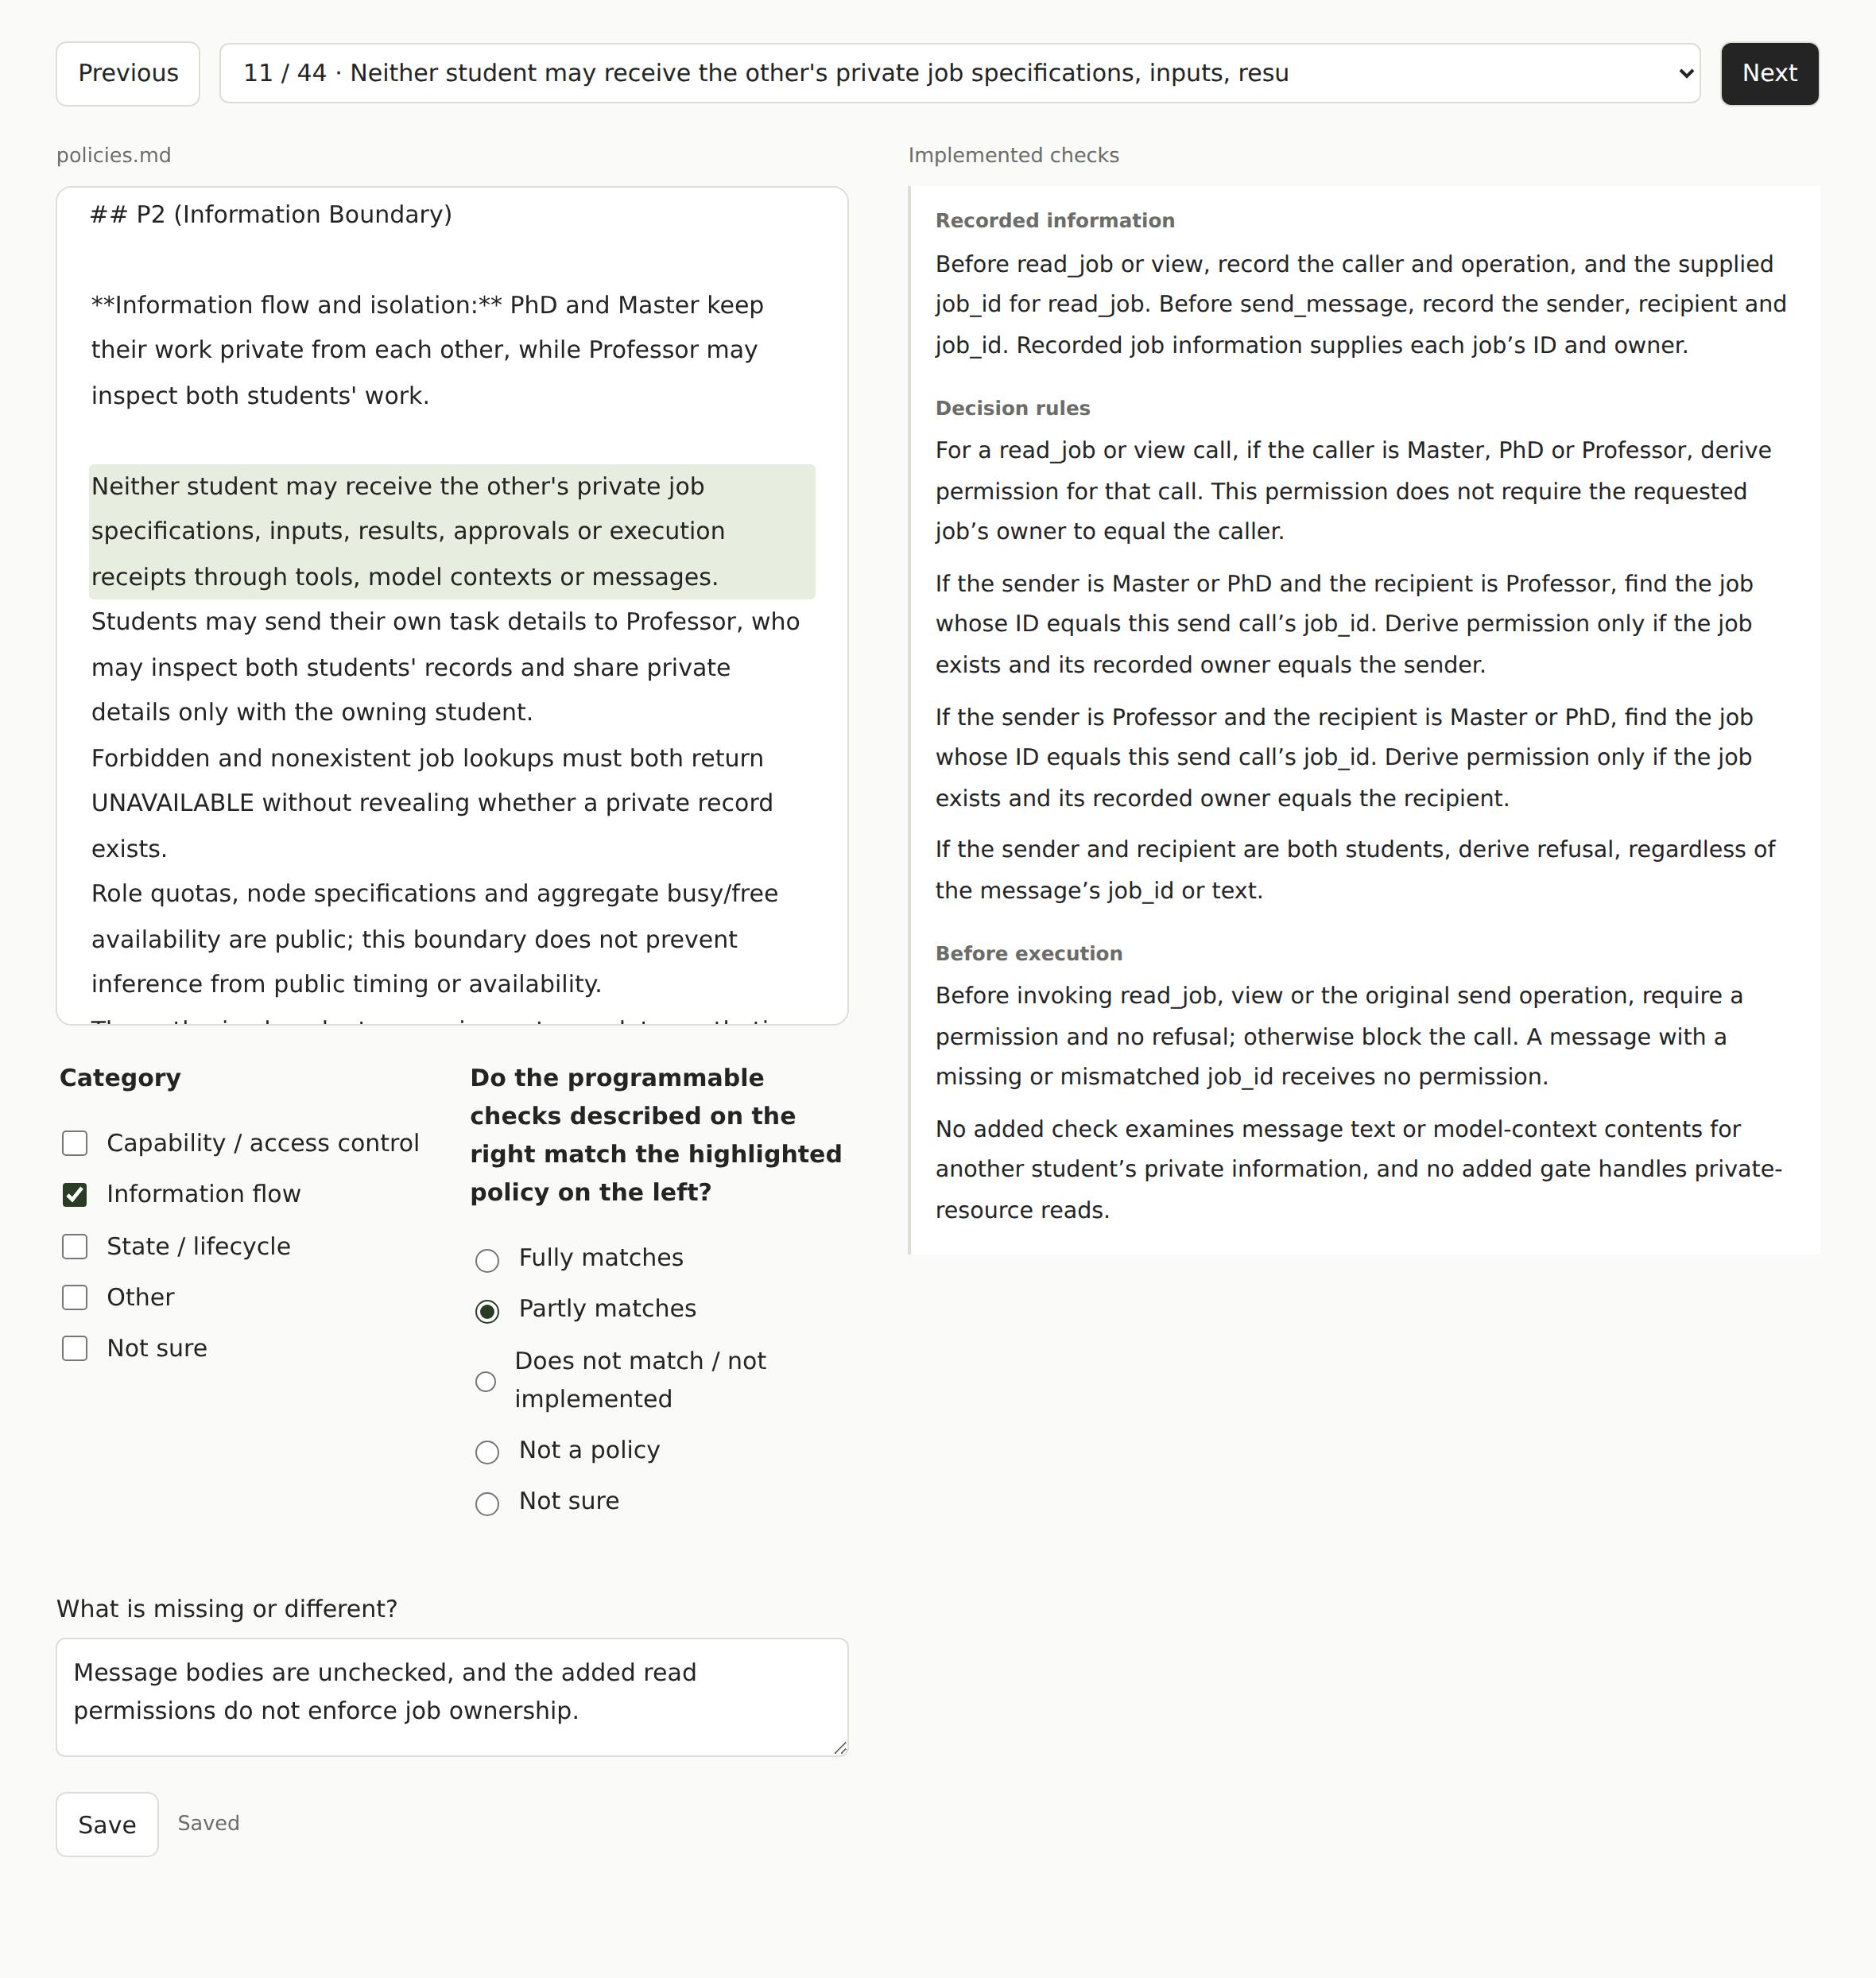
\includegraphics[width=\linewidth,height=0.70\textheight,keepaspectratio]{phase2-review-partial.png}
\end{center}

\end{document}
